% Options for packages loaded elsewhere
\PassOptionsToPackage{unicode}{hyperref}
\PassOptionsToPackage{hyphens}{url}
\PassOptionsToPackage{dvipsnames,svgnames,x11names}{xcolor}
%
\documentclass[
  super,
  preprint,
  3p]{elsarticle}

\usepackage{amsmath,amssymb}
\usepackage{iftex}
\ifPDFTeX
  \usepackage[T1]{fontenc}
  \usepackage[utf8]{inputenc}
  \usepackage{textcomp} % provide euro and other symbols
\else % if luatex or xetex
  \usepackage{unicode-math}
  \defaultfontfeatures{Scale=MatchLowercase}
  \defaultfontfeatures[\rmfamily]{Ligatures=TeX,Scale=1}
\fi
\usepackage{lmodern}
\ifPDFTeX\else  
    % xetex/luatex font selection
\fi
% Use upquote if available, for straight quotes in verbatim environments
\IfFileExists{upquote.sty}{\usepackage{upquote}}{}
\IfFileExists{microtype.sty}{% use microtype if available
  \usepackage[]{microtype}
  \UseMicrotypeSet[protrusion]{basicmath} % disable protrusion for tt fonts
}{}
\makeatletter
\@ifundefined{KOMAClassName}{% if non-KOMA class
  \IfFileExists{parskip.sty}{%
    \usepackage{parskip}
  }{% else
    \setlength{\parindent}{0pt}
    \setlength{\parskip}{6pt plus 2pt minus 1pt}}
}{% if KOMA class
  \KOMAoptions{parskip=half}}
\makeatother
\usepackage{xcolor}
\setlength{\emergencystretch}{3em} % prevent overfull lines
\setcounter{secnumdepth}{5}
% Make \paragraph and \subparagraph free-standing
\ifx\paragraph\undefined\else
  \let\oldparagraph\paragraph
  \renewcommand{\paragraph}[1]{\oldparagraph{#1}\mbox{}}
\fi
\ifx\subparagraph\undefined\else
  \let\oldsubparagraph\subparagraph
  \renewcommand{\subparagraph}[1]{\oldsubparagraph{#1}\mbox{}}
\fi

\usepackage{color}
\usepackage{fancyvrb}
\newcommand{\VerbBar}{|}
\newcommand{\VERB}{\Verb[commandchars=\\\{\}]}
\DefineVerbatimEnvironment{Highlighting}{Verbatim}{commandchars=\\\{\}}
% Add ',fontsize=\small' for more characters per line
\usepackage{framed}
\definecolor{shadecolor}{RGB}{241,243,245}
\newenvironment{Shaded}{\begin{snugshade}}{\end{snugshade}}
\newcommand{\AlertTok}[1]{\textcolor[rgb]{0.68,0.00,0.00}{#1}}
\newcommand{\AnnotationTok}[1]{\textcolor[rgb]{0.37,0.37,0.37}{#1}}
\newcommand{\AttributeTok}[1]{\textcolor[rgb]{0.40,0.45,0.13}{#1}}
\newcommand{\BaseNTok}[1]{\textcolor[rgb]{0.68,0.00,0.00}{#1}}
\newcommand{\BuiltInTok}[1]{\textcolor[rgb]{0.00,0.23,0.31}{#1}}
\newcommand{\CharTok}[1]{\textcolor[rgb]{0.13,0.47,0.30}{#1}}
\newcommand{\CommentTok}[1]{\textcolor[rgb]{0.37,0.37,0.37}{#1}}
\newcommand{\CommentVarTok}[1]{\textcolor[rgb]{0.37,0.37,0.37}{\textit{#1}}}
\newcommand{\ConstantTok}[1]{\textcolor[rgb]{0.56,0.35,0.01}{#1}}
\newcommand{\ControlFlowTok}[1]{\textcolor[rgb]{0.00,0.23,0.31}{#1}}
\newcommand{\DataTypeTok}[1]{\textcolor[rgb]{0.68,0.00,0.00}{#1}}
\newcommand{\DecValTok}[1]{\textcolor[rgb]{0.68,0.00,0.00}{#1}}
\newcommand{\DocumentationTok}[1]{\textcolor[rgb]{0.37,0.37,0.37}{\textit{#1}}}
\newcommand{\ErrorTok}[1]{\textcolor[rgb]{0.68,0.00,0.00}{#1}}
\newcommand{\ExtensionTok}[1]{\textcolor[rgb]{0.00,0.23,0.31}{#1}}
\newcommand{\FloatTok}[1]{\textcolor[rgb]{0.68,0.00,0.00}{#1}}
\newcommand{\FunctionTok}[1]{\textcolor[rgb]{0.28,0.35,0.67}{#1}}
\newcommand{\ImportTok}[1]{\textcolor[rgb]{0.00,0.46,0.62}{#1}}
\newcommand{\InformationTok}[1]{\textcolor[rgb]{0.37,0.37,0.37}{#1}}
\newcommand{\KeywordTok}[1]{\textcolor[rgb]{0.00,0.23,0.31}{#1}}
\newcommand{\NormalTok}[1]{\textcolor[rgb]{0.00,0.23,0.31}{#1}}
\newcommand{\OperatorTok}[1]{\textcolor[rgb]{0.37,0.37,0.37}{#1}}
\newcommand{\OtherTok}[1]{\textcolor[rgb]{0.00,0.23,0.31}{#1}}
\newcommand{\PreprocessorTok}[1]{\textcolor[rgb]{0.68,0.00,0.00}{#1}}
\newcommand{\RegionMarkerTok}[1]{\textcolor[rgb]{0.00,0.23,0.31}{#1}}
\newcommand{\SpecialCharTok}[1]{\textcolor[rgb]{0.37,0.37,0.37}{#1}}
\newcommand{\SpecialStringTok}[1]{\textcolor[rgb]{0.13,0.47,0.30}{#1}}
\newcommand{\StringTok}[1]{\textcolor[rgb]{0.13,0.47,0.30}{#1}}
\newcommand{\VariableTok}[1]{\textcolor[rgb]{0.07,0.07,0.07}{#1}}
\newcommand{\VerbatimStringTok}[1]{\textcolor[rgb]{0.13,0.47,0.30}{#1}}
\newcommand{\WarningTok}[1]{\textcolor[rgb]{0.37,0.37,0.37}{\textit{#1}}}

\providecommand{\tightlist}{%
  \setlength{\itemsep}{0pt}\setlength{\parskip}{0pt}}\usepackage{longtable,booktabs,array}
\usepackage{calc} % for calculating minipage widths
% Correct order of tables after \paragraph or \subparagraph
\usepackage{etoolbox}
\makeatletter
\patchcmd\longtable{\par}{\if@noskipsec\mbox{}\fi\par}{}{}
\makeatother
% Allow footnotes in longtable head/foot
\IfFileExists{footnotehyper.sty}{\usepackage{footnotehyper}}{\usepackage{footnote}}
\makesavenoteenv{longtable}
\usepackage{graphicx}
\makeatletter
\def\maxwidth{\ifdim\Gin@nat@width>\linewidth\linewidth\else\Gin@nat@width\fi}
\def\maxheight{\ifdim\Gin@nat@height>\textheight\textheight\else\Gin@nat@height\fi}
\makeatother
% Scale images if necessary, so that they will not overflow the page
% margins by default, and it is still possible to overwrite the defaults
% using explicit options in \includegraphics[width, height, ...]{}
\setkeys{Gin}{width=\maxwidth,height=\maxheight,keepaspectratio}
% Set default figure placement to htbp
\makeatletter
\def\fps@figure{htbp}
\makeatother

\makeatletter
\makeatother
\makeatletter
\makeatother
\makeatletter
\@ifpackageloaded{caption}{}{\usepackage{caption}}
\AtBeginDocument{%
\ifdefined\contentsname
  \renewcommand*\contentsname{Table of contents}
\else
  \newcommand\contentsname{Table of contents}
\fi
\ifdefined\listfigurename
  \renewcommand*\listfigurename{List of Figures}
\else
  \newcommand\listfigurename{List of Figures}
\fi
\ifdefined\listtablename
  \renewcommand*\listtablename{List of Tables}
\else
  \newcommand\listtablename{List of Tables}
\fi
\ifdefined\figurename
  \renewcommand*\figurename{Figure}
\else
  \newcommand\figurename{Figure}
\fi
\ifdefined\tablename
  \renewcommand*\tablename{Table}
\else
  \newcommand\tablename{Table}
\fi
}
\@ifpackageloaded{float}{}{\usepackage{float}}
\floatstyle{ruled}
\@ifundefined{c@chapter}{\newfloat{codelisting}{h}{lop}}{\newfloat{codelisting}{h}{lop}[chapter]}
\floatname{codelisting}{Listing}
\newcommand*\listoflistings{\listof{codelisting}{List of Listings}}
\makeatother
\makeatletter
\@ifpackageloaded{caption}{}{\usepackage{caption}}
\@ifpackageloaded{subcaption}{}{\usepackage{subcaption}}
\makeatother
\makeatletter
\@ifpackageloaded{tcolorbox}{}{\usepackage[skins,breakable]{tcolorbox}}
\makeatother
\makeatletter
\@ifundefined{shadecolor}{\definecolor{shadecolor}{rgb}{.97, .97, .97}}
\makeatother
\makeatletter
\makeatother
\makeatletter
\makeatother
\journal{Ecological Indicators}
\ifLuaTeX
  \usepackage{selnolig}  % disable illegal ligatures
\fi
\usepackage[]{natbib}
\bibliographystyle{elsarticle-num}
\IfFileExists{bookmark.sty}{\usepackage{bookmark}}{\usepackage{hyperref}}
\IfFileExists{xurl.sty}{\usepackage{xurl}}{} % add URL line breaks if available
\urlstyle{same} % disable monospaced font for URLs
\hypersetup{
  pdftitle={Using spatially biased variables in ecosystem condition accounting with a GIS based workflow},
  pdfauthor={Anders Lorentzen Kolstad; Bob Security; Cat Memes; Derek Zoolander},
  pdfkeywords={SEEA EA, alien species},
  colorlinks=true,
  linkcolor={blue},
  filecolor={Maroon},
  citecolor={Blue},
  urlcolor={Blue},
  pdfcreator={LaTeX via pandoc}}

\setlength{\parindent}{6pt}
\begin{document}

\begin{frontmatter}
\title{Using spatially biased variables in ecosystem condition
accounting with a GIS based workflow \\\large{A Short Subtitle} }
\author[1]{Anders Lorentzen Kolstad%
\corref{cor1}%
\fnref{fn1}}
 \ead{anders.kolstad@nina.no} 
\author[2]{Bob Security%
%
\fnref{fn2}}
 \ead{bob@example.com} 
\author[2]{Cat Memes%
%
\fnref{fn3}}
 \ead{cat@example.com} 
\author[]{Derek Zoolander%
%
}
 \ead{derek@example.com} 

\affiliation[1]{organization={Norwegian Institute for Nature
Research, Department of Terrestrial Ecology},addressline={Street
Address},city={City},postcode={Postal Code},postcodesep={}}
\affiliation[2]{organization={Another University, Department
Name},addressline={Street Address},city={City},postcode={Postal
Code},postcodesep={}}

\cortext[cor1]{Corresponding author}
\fntext[fn1]{This is the first author footnote.}
\fntext[fn2]{Another author footnote, this is a very long footnote and
it should be a really long footnote. But this footnote is not yet
sufficiently long enough to make two lines of footnote text.}
\fntext[fn3]{Yet another author footnote.}

        
\begin{abstract}
This is the abstract. Lorem ipsum dolor sit amet, consectetur adipiscing
elit. Vestibulum augue turpis, dictum non malesuada a, volutpat eget
velit. Nam placerat turpis purus, eu tristique ex tincidunt et. Mauris
sed augue eget turpis ultrices tincidunt. Sed et mi in leo porta
egestas. Aliquam non laoreet velit. Nunc quis ex vitae eros aliquet
auctor nec ac libero. Duis laoreet sapien eu mi luctus, in bibendum leo
molestie. Sed hendrerit diam diam, ac dapibus nisl volutpat vitae.
Aliquam bibendum varius libero, eu efficitur justo rutrum at. Sed at
tempus elit.
\end{abstract}





\begin{keyword}
    SEEA EA \sep 
    alien species
\end{keyword}
\end{frontmatter}
    \ifdefined\Shaded\renewenvironment{Shaded}{\begin{tcolorbox}[boxrule=0pt, frame hidden, borderline west={3pt}{0pt}{shadecolor}, interior hidden, enhanced, sharp corners, breakable]}{\end{tcolorbox}}\fi

\hypertarget{introduction}{%
\section{Introduction}\label{introduction}}

Some general text about the decline in natural capital?

Ecosystem condition accounting is the game of compiling relevant data on
the status, trends and qualities of ecosystems (i.e.~nature) and
communicating this in a structured format. Its purpose is to make it
easier to account for nature in policy by making the environmental costs
of certain policies and practices visible to decision makers. As natural
capital keeps declining all over the world, it is becoming increasingly
urgent to make the message clear to decision makers about A statistical
standard for ecosystem accounting, including ecosystem condition
accounting, was developed by the UN and adopted by the UN Statistical
Commission in 2021 and is called SEEA EA (System of
Environmental-Economic Accounting - Ecosystem Accounting). The standard,
or framework, is a set of rules, principles and best practices for
compiling Ecosystem accounts, mainly aimed at national accounts.

Central to ecosystem condition accounts are variables and indicators.
These are parameters chosen to reflect the sentral condition
characteristics of the ecosystems, and that can be quantified and
ideally monitored over time to reflect the status and trends in
condition. Indicators are (data) variables that are normalised
(rescaled) against upper and lower reference values to become bound
between the values 0 and 1. This normalisation ensures that indicators
are more comparable because an indicator value of 1 will mean the same
for all indicators, i.e.~that the variable equals the upper reference
value which again reflect the value of the variables under the reference
condition. Similarly, a value of 0 mean that the variable is the worst
possible state. The reference condition needs to be defined for each
Ecosystem Condition Assessment separately, but SEEA EA gives some
suggestion, such as an an ecosystem with no or minimal anthorpogenic
disturbance.

A general requirement for indicators in the SEEA EA framework is that
they should give an unbiased representation of the condition inside the
ecosystem assets (Czucz et al 2021; Table 1 - validity; see also SEEA EA
§2.87) Ecosystem assets are defined as ``ecological entities {[}meaning
areas{]} about which information is sought and about which statistics
are ultimately compiled (REF). This requirement for indicator validity
means that spatially biased data are ill suited, especially if sampling
intensity varies along gradient of anthropogenic pressures and hence
ecosystem condition. SEEA EA is spatially explicit, which in practice
means that indicators that are in some way sampled (i.e.~not complete
wall-to-wall data like remotely sensed imagery), the values are
projected on to areas on the map, so that all areas inside the ecosystem
accounting area get assigned value for that indicator. There are at
least 3 general ways to achieve this complete areal coverage of
indicator values:

\begin{enumerate}
\def\labelenumi{\alph{enumi}.}
\tightlist
\item
  Using wall-to-wall data (e.g.~remotely sensed data)
\item
  Predict values using a model (e.g.~by accounting for environmental
  variation)
\item
  Simple projection of some best estimate, typically a central tendency
  from area representative data
\end{enumerate}

The need for an unbiased estimation of indicator values is
unquestionable, but nonetheless, this requirement puts a large
limitation on what types of data one can use. Ecosystem condition
assessments are generally limited by data availability, and the choice
of variables and indicators to include in assessments are more often or
not a pragmatic and opportunistic one which is unlikely to reflect the
full scope of the ecosystem condition characteristics. Note that the
same is true for thematic biases. For example reflected in the scarcity
of data included on insects or soil biota, even though most will agree
they represent key ecosystem characteristics. Also having data from only
one or a subset of nature types inside what is defined as the ecosystem
in the assessment, is a typical thematic bias in ecosystem accounting.
However, in this paper we chose to focus on spatial bias.

Being able to make use of spatially biased data would greatly alleviate
data shortage problems in ecosystem condition accounts. One way to
achieve this is modelling (option b in the list above). Models can
describe the general associations between the spatially sampled data and
the context (e.g.~the set of environmental variables) where it was
samples, and use these arelationships to predict and project indicator
values to areas that where not originally sampled. Depending on the data
that goes into these models, they can be very reliable and make good
indicators. This is especially true when the ecosystem assets are large
(e.g.~regions or nations). But when they are small, like the scale of a
municipality, and when the indicator is more likely to be used as the
evidence base in concrete physical land use planning, then the inherent
lvel of uncertainty from such models becomes unacceptable.

In this study we explore the potential for using a stratified
aggregation technique to make use of spatially biased field data in
ecosystem condition accounting. We demonstrate this technique using a
generic GIS-based workflow for compiling ecosystem condition accounts
that can be applied at any spatial scale, and we highlight the
opportunities for local use-cases of this workflow by contrasting our
findings across four neighboring municipalities in Norway. The main
question is how much generalisation can we perform on the data we have
before the resulting indicator looses its practical value in local
governance processes. We end by interviewing end-users from the relevant
municipalities about the perceived benefits and shortcomings of our
condition indicators.

\hypertarget{material-and-methods}{%
\section{Material and Methods}\label{material-and-methods}}

In this study we focused on open mire ecosystems in Norway. For this
ecosystem we have an ecosystem delineation map produced using remotely
sensed data and a deep learning model (REF Bakkestuen). This model,
which has a 90.9\% precision when tested against independent field data,
estimates 12.7\% of the area in southern Norway is mire (Bakkestuen
REF). Mires are ecologically and socially important in Norway simply do
to its large extent, and due to its role in climate mitigation, as mires
store a large amount of carbon (REF?). There has not been a national
assessment of the ecosystem condition of mires in Norway, but we recent
contributed on a report which presented several new indicators that can
be used in future assessment (REF Nybø, and web site). This study builds
on the work in that report.

We started by defining the reference state as one where ecosystems are
subject to little or no human influence, with a climate as in the period
1961-1990 and a native species pool similar as today (i.e no mammoths
allowed). We then identified two \emph{ecosystem condition
characteristics} that, along with many other characteristics that we do
not specify here, define the typical behavior of open mire ecosystems in
the reference condition: species composition, and; vegetation
intactness.

To describe these two concepts we use five condition variables from the
same data set (see Table~\ref{tbl-variables}.

\hypertarget{tbl-variables}{}
\begin{longtable}[]{@{}
  >{\raggedright\arraybackslash}p{(\columnwidth - 8\tabcolsep) * \real{0.2000}}
  >{\raggedright\arraybackslash}p{(\columnwidth - 8\tabcolsep) * \real{0.2000}}
  >{\raggedright\arraybackslash}p{(\columnwidth - 8\tabcolsep) * \real{0.2000}}
  >{\raggedright\arraybackslash}p{(\columnwidth - 8\tabcolsep) * \real{0.2000}}
  >{\raggedright\arraybackslash}p{(\columnwidth - 8\tabcolsep) * \real{0.2000}}@{}}
\caption{\label{tbl-variables}Variables used in this
study}\tabularnewline
\toprule\noalign{}
\begin{minipage}[b]{\linewidth}\raggedright
Variable code
\end{minipage} & \begin{minipage}[b]{\linewidth}\raggedright
Variable name
\end{minipage} & \begin{minipage}[b]{\linewidth}\raggedright
Measurement unit
\end{minipage} & \begin{minipage}[b]{\linewidth}\raggedright
Description
\end{minipage} & \begin{minipage}[b]{\linewidth}\raggedright
Reference
\end{minipage} \\
\midrule\noalign{}
\endfirsthead
\toprule\noalign{}
\begin{minipage}[b]{\linewidth}\raggedright
Variable code
\end{minipage} & \begin{minipage}[b]{\linewidth}\raggedright
Variable name
\end{minipage} & \begin{minipage}[b]{\linewidth}\raggedright
Measurement unit
\end{minipage} & \begin{minipage}[b]{\linewidth}\raggedright
Description
\end{minipage} & \begin{minipage}[b]{\linewidth}\raggedright
Reference
\end{minipage} \\
\midrule\noalign{}
\endhead
\bottomrule\noalign{}
\endlastfoot
7FK & Prevalence of alien species & Unitless, ordinal, non-linear scale
from 1 (no alien species) to 7 (only alien species) & The fraction of
the species composition made up from alien species & Halvorsen \\
7SE & Human caused abration or abration-caused erosion & Unitless,
ordinal, non-linear scale from 1 to 4. & Measures the frequency of
imagined 4 m\textsuperscript{2} quadrats layed over the area that has
some sign of abration & ref \\
PRSL & \emph{as above} & Unitless, ordinal, non-linear scale from 0 to
7. & Same as 7SE, but recorded at a higher resolution & Mdir \\
7TK & Tracks from large vehicles & Unitless, ordinal, non-linear scale
from 1 to 4. & Measures the frequency of imagined 100
m\textsuperscript{2} quadrats layed over the area that has some signs of
vehicle tracks & Halvorsen \\
PRTK & \emph{as above} & Unitless, ordinal, non-linear scale from 0 to
7. & Same as 7TK, but recorded at a higher resolution & Mdir \\
Infrastructure Index & Infrastructure Index & Unitelss linear scale from
0 to 13.2 & Unitelss index ranging from from 0 to 13.2 & Erikstad \\
HIA & Human Impact area & Ordinal, non-linear scale from 1 to 4 & A
categorical representation of the infrastructure index & this paper \\
\end{longtable}

Reference to Figure~\ref{fig-carsplot}

\begin{Shaded}
\begin{Highlighting}[]
\FunctionTok{plot}\NormalTok{(cars)}
\end{Highlighting}
\end{Shaded}

\begin{figure}[H]

{\centering 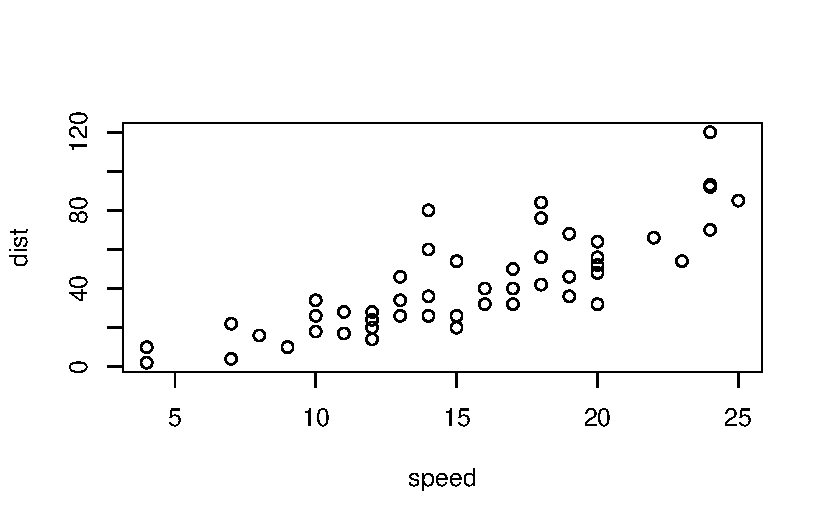
\includegraphics{HIAs_files/figure-pdf/fig-carsplot-1.pdf}

}

\caption{\label{fig-carsplot}Test caption}

\end{figure}

The data set is from a standardised field survey of nature types in
Norway that started in 2018 and which is still ongoing (REF). We
included data fram 2018 to 2023. In this survey, selected nature types
are delineatied on a map, and each locality is scored on a range of
variables relevant for describing the state and quality of nature. The
surveys are commissioned with the goal of producing data relevant for
immediate land-use decisions, and is therefore spatially biased,
typically towards areas with high human impact or expected impact. In
addition there is a thematic and size bias in the sampling protocol. Of
all possible mire types, the survey only maps the following:

\begin{itemize}
\item
  Southern ombrotrophic mires \textgreater{} 2500 m\textsuperscript{2}
\item
  Northern omgrotrophic \textgreater{} 10.000 m\textsuperscript{2}
\item
  All semi-natural mires (minerotrophic)
\item
  Calcareous southern fens \textgreater500 m\textsuperscript{2}
\item
  Calcareous northen fens \textgreater1000 m\textsuperscript{2}
\end{itemize}

In the above, \emph{southern} refers to boreonemoral and southboreal
zones, and \emph{northern} refers to mid-boreal, north boreal, and
alpine zones. In addition, the northern fens need to be even more
calcareous than the southern fens in order to be surveyed. In this paper
we assume the survey is representative for the entire mire ecosystem in
Norway. Although it is possible that smaller or less calcareous mires
will score systematically different than the ones that are surveyed we
do not think this is the case for our variables at least.

7FK was developed into a single indicator (i.e.~a normalised variable)
named \emph{Alien plant cover}. Variables 2-5 describe very related
aspects as so they where planned to be combined into one indicator
called antropogenic disturbance to soil and vegetation, or ADSV for
short. This was done by taking the value from the variable with the
lowest value, i.e.~worst condition. For both indicators, the lower and
upper reference values, i.e.~the worst and best possible condition that
the variables can be in, is given by the range of the data where 0 or 1
is the lower limit and 4, 7 or 8 is the upper limit, depending on the
variable (see Table~\ref{tbl-variables}).

The Alien plant cover was assigned to ECT class B1 - Compositional state
characteristics and ADSV was assigned to ECT class A1 - Physical state
characteristics (REF).

\begin{figure}

{\centering \includegraphics{../images/workflow.jpg}

}

\caption{\label{fig-workflow}Schematic workflow followed in this paper.
Sub-index A is calculated using spatially explicit aggregation (i.e .a
simple overlay takingthe mean value).}

\end{figure}

We chose three municipalities in Norway to test out the indicator (FIG).
These municipalities are spread over xxx km north to south, and also
differ in the amount of mire area, the total area surveyed, and the
prevalence of infrastructure (TABLE)

To

Validation/sensitivity analyses (varying HIA resolution and minimum
\emph{n}?)

Schematic GIS workflow, see Figure~\ref{fig-workflow}

Aggregation

\hypertarget{results}{%
\section{Results}\label{results}}

Data availability/coverage

Validation

National/regional indicator - do we have enough data?

Municipal case study

\hypertarget{discussion}{%
\section{Discussion}\label{discussion}}

\hypertarget{conclusion}{%
\section{Conclusion}\label{conclusion}}

\hypertarget{credit-authorship-contribution-statement}{%
\section*{Credit authorship contribution
statement}\label{credit-authorship-contribution-statement}}
\addcontentsline{toc}{section}{Credit authorship contribution statement}

\hypertarget{declaration-of-competing-interest}{%
\section*{Declaration of Competing
Interest}\label{declaration-of-competing-interest}}
\addcontentsline{toc}{section}{Declaration of Competing Interest}

\hypertarget{acknowledgements}{%
\section*{Acknowledgements}\label{acknowledgements}}
\addcontentsline{toc}{section}{Acknowledgements}

\hypertarget{data-availability}{%
\section*{Data availability}\label{data-availability}}
\addcontentsline{toc}{section}{Data availability}


\renewcommand\refname{References}
  \bibliography{bibliography.bib}


\end{document}
